\documentclass[12pt]{article}
\usepackage{graphicx} % Required for inserting images
\usepackage{soul}
\usepackage{color}
\usepackage{hyperref}
\usepackage[affil-it]{authblk}
\title{\textbf{Predicción de los precios de la vivienda en Bogotá: Problem Set 2}}
\author{Lina Maria Bautista}
\author{Juan Pablo Bermudez}
\author{Esteban Meza}
\author{Pharad Sebastián Escobar}
\affil{}
\date{30 de Octubre de 2023}

\usepackage{blindtext}
\usepackage[T1]{fontenc}
\usepackage{multicol}
\usepackage[utf8]{inputenc}
\usepackage[spanish]{babel}

\usepackage{amsthm}

\usepackage{amssymb}
\usepackage{amsmath}
\usepackage{graphicx}
\usepackage{stackengine}
\usepackage{listings}
\usepackage{float}


\usepackage{array, multicol, multirow, makecell} 
\usepackage{graphicx, wrapfig, lscape, rotating, float, booktabs} 
\usepackage[usenames,dvipsnames,svgnames,table]{xcolor} 
\usepackage{tabularx} 
\usepackage{tabulary}
\usepackage{subfig}
\usepackage[usenames,dvipsnames,svgnames,table]{xcolor} 
\usepackage{tabularx} 
\usepackage{tabulary} 
\usepackage{hyperref}
\setlength{\parindent}{0pt}
\usepackage[left=2.5cm,right=2.5cm,top=2.5cm,bottom=2.5cm]{geometry}
\usepackage[labelfont=bf,font=small,justification=justified]{caption}[2008/04/01]
\DeclareCaptionLabelSeparator{punto}{. }
\usepackage{enumerate}



\begin{document}

\maketitle
El repositorio del presente trabajo se encuentra en el siguiente URL \href{https://github.com/jbermudezc01/Problem_set2_BDML}{github.com/jbermudezc01/}.
\section{Introducción}
En el contexto dinámico del mercado inmobiliario en Bogotá, las empresas del sector encuentran relevante calcular de manera precisa los precios de las viviendas, especialmente a la luz de experiencias pasadas. La empresa Zillow ejemplifica esta necesidad, pues sus algoritmos generaron predicciones sobrestimadas que resultaron en pérdidas aproximadas de 500 millones de dólares y una reducción del 25\% de su fuerza laboral. En este sentido, la visión de nuestro cliente es maximizar su adquisición de propiedades en el sector de Chapinero, todo ello bajo la restricción de su presupuesto. Por esta razón, el propósito del presente texto es diseñar un modelo predictivo que no solo supere los desafíos técnicos, sino que también se alinee con la visión de nuestro cliente.\\

Los autores Cabrera-Rodríguez, W., Mariño-Montaña, J. y Quicazán-Moreno (2019), plantean un referente académico pionero en la incorporación de variables espaciales en modelos hedónicos. Esto les permitió obtener una ventaja sobre los índices calculados en esa época para la ciudad de Bogotá, que utilizaban variables de estratificación o métodos hedónicos sin considerar variables espaciales. Por un lado, esta experiencia es relevante para el presente estudio, ya que resalta la importancia de las características de las viviendas en la estimación de sus precios. Por otro lado, debido a los objetivos predictivos de la presente investigación, se proponen modelos de machine learning como Regresión Lineal, Ridge, Lasso, Elastic Net,
CART, Random Forest o Boosting. Por lo tanto, utilizaremos una base de datos con 48,930 observaciones y 148 variables, de las cuales más de 100 reflejan características espaciales de las viviendas. El presente estudio encuentra que el método de boosting es una herramienta efectiva y adaptable para la predicción de precios de viviendas debido a su capacidad de aprendizaje, su capacidad para lidiar con datos faltantes y valores inusuales, y su desempeño generalmente consistente en diversos contextos.\\

De esta manera, el presente texto se divide en tres secciones principales. En primer lugar, se realiza una descripción del proceso de recolección de los datos y posteriormente se presentan las estadísticas descriptivas de dichos datos, denotando así la relevancia de cada una de las variables incluidas en el set de datos.\\

En segundo lugar, se propone el modelo a utilizar y sus resultados, en el caso del presente trabajo, un Boosting con 114 árboles, penalidad de 0.001 y profundidad de árbol 1.\\

Finalmente, se presentan las conclusiones y recomendaciones en las que se hace referencia a la necesidad de una mayor recolección de datos por parte de la compañía, además de aclarar que se corrieron modelos con el fin de reducir la cantidad de predictores, sin embargo, la que presento mayor rendimiento en la predicción seguía siendo la de boosting con los 148 predictores, denotando así que las variables dentro del modelo eran relevantes en el ajuste y predicción de wste.

\section{Datos}
\subsection{Creación de la base de datos}
La información proveída para el presente trabajo se constituía por dos bases de datos que contenían información de propiedades en Chapinero, sus precios y  características. Estas bases de datos se habían clasificado bajo el criterio de si los datos hacían parte del conjunto de entrenamiento o prueba. Con el fin de poder tratar estos datos de forma más fácil, se juntaron en una única base de datos uniendolas por filas. Aquí se creo una nueva variable que pudiera indicar a qué conjunto pertenecía cada una de las observaciones, si a train (entrenamiento) o test (prueba). Al finalizar este proceso se consiguió una base de datos de 48930 observaciones, 21,02\% (10286) de ellas como conjunto de prueba y 79\% (38644) de ellas como conjunto de entrenamiento.\\

Esta primera base de datos agregada contenía información para la identificación de la propiedad, la ciudad, el precio, información del año y el mes en el que la información fue recolectada, superficie total y cubierta de la propiedad, número de cuartos, habitaciones, baños, una breve descripción de la propiedad y las coordenadas de ubicación de cada una de ellas. \\

La mayoría de estas variables contenían una gran cantidad de NAs, por lo que debieron ser sometidas a diferentes procesos para poder reducir al máximo la cantidad de datos faltantes. Para el número de baños se imputó por la moda (bathrooms). En el caso del número de cuartos (bedrooms) y el número de piso (piso\_numerico), se extrajeron de la  descripción. En el caso de no poder encontrarlos dentro del texto se imputaron por la moda de la variable agrupada según el tipo de propiedad.\\ 

La forma en la que venían escritos los datos para "bedroom" hizo que se recolectaran muchos datos atípicos por lo que se decidió trabajar solo con la variable "rooms" reemplazando los faltantes por la moda. \\

Por otra parte, a partir de la descripción también se extrajó información para la variable de superficie "surface", ya que la mayoría de las propiedades indicaban su área total y cubierta, aquellas en las que no se pudo realizar la extracción, se imputaron por la media de la superficie agrupada por número de cuartos. Es decir, de las observaciones con la misma cantidad de cuartos, se extrajo la media de la superficie.\\

A pesar de que estas variables proveían mucha información que podía afectar el precio de una propiedad, era necesario crear nuevas variables que pudieran ser indicativas de características de la propiedad, para esto se recurrió nuevamente a los textos de descripción de las propiedades, de donde se crearon
variables para indicar si las propiedades contaban con parqueadero, terraza, ascensor, vigilancia, depósito, cocina integral o piso laminado. Todas estas variables incluidas como dummys que indicaban la presencia de la característica o no.\\

Más allá de las características intrínsecas de un inmueble, es necesario observar otro tipo de variables que pueden afectar el precio de este, ejemplo de ello es la cercanía de las propiedades a lugares de interes como parques, museos, hospitales, universidades, atractivos turísticos y otros ammenities que pueden afectar positivamente el precio. Empero, otras características como la cercanía  a bares y clubes pueden ser determinantes de la reducción de los precios de los inmuebles, específicamente cuando se trata la localidad de Chapinero en donde se pueden encontrar diferentes puntos de interés de entretenimiento.\\

Para poder extraer este tipo de aspectos se recurrió a la API de Open Street Maps que permite acceder a información espacial de estos lugares. Esta API funciona a través de etiquetas y llaves que indican cada una de estas variables. \\

Con el fin de poder extraer la mayor cantidad de información posible, se extrajeron las coordenadas de dos llaves principales: "ammenities" y "leisure", entre ellas contenían información espacial para cerca de 100 etiquetas (variables). Asimismo, de la llave \textit{shop} se recolectó información epacial de centros comerciales; de la llave \textit{highway} se extrajo información para vías de bicicletas; y de la llave \textit{landuse"} se adquirió información para establecimientos comerciales.\\

Otro aspecto que se consideró fundamental para la determinación de los precios de los inmuebles en Chapinero fue la cercanía a estaciones de SITP y transmilenio. Para poder acceder a esta información se recurrió a los datos abiertos de transmilenio para adquirir la latitud y longitud de cada una de las estaciones, descargando los archivos en formato. json.\\

Asimismo, para recolectar una mayor cantidad de información sobre los predios, se tomaron algunas bases de datos abiertos de Bogotá, de donde se extrajeron variables  espaciales de la ubiación de localidad, UPZ y manzana en la que se encontraba cada predio y el estrato, además de el valor de referencia catastral, la cantidad de predios y área construida por manzana.\\

Posteriormente, con el fin de darle mayor complejidad a los modelos se introdujeron algunas variables de interacción entre el estrato y las distancias de algunos lugares de interés como universidades, restaurantes, entre otros.\\

Finalmente, se construyó una base de datos que incluye 48930 observaciones y 148 variables. Para interés del lector se hace referencia a que se puede acceder a los datos a través del \href{https://github.com/jbermudezc01/Problem_set2_BDML}{repositorio} de github en el que se encuentra bajo el nombre de "Datos\_limpios.RData".\\


\subsection{ Estadisticas descriptivas }

\begin{table}
\centering
\caption{Características internas de las viviendas}
\label{tab:caracteristicas_internas}
\begin{tabular}{|l|r|r|}
\hline
Nombre variable &  Apartamento &   Casa \\
\hline
Moda de rooms                    &         3.00 &   3.00 \\
Moda de bedrooms                 &         3.00 &   4.00 \\
Moda de bathrooms                &         2.00 &   3.00 \\
Moda de piso\_numerico            &         2.00 &   1.00 \\
Proporción tiene parqueadero     &         0.72 &   0.58 \\
Proporción tiene terraza         &         0.47 &   0.27 \\
Proporción tiene ascensor        &         0.23 &   0.02 \\
Proporción tiene vigilancia      &         0.28 &   0.12 \\
Proporción tiene deposito        &         0.40 &   0.20 \\
Proporción tiene cocina\_integral &         0.25 &   0.27 \\
Proporción tiene piso\_laminado   &         0.03 &   0.01 \\
Promedio surface\_total\_kkn       &       121.78 & 218.49 \\
\hline
\end{tabular}
\end{table}


La Tabla \ref{tab:caracteristicas_internas} proporciona una comparativa interesante entre apartamentos y casas en términos de sus características internas predominantes. Observamos que tanto en casas como en apartamentos, la moda de habitaciones y dormitorios es de 3, lo que sugiere que estas propiedades suelen diseñarse para familias pequeñas o medianas. Sin embargo, las casas tienden a tener un dormitorio adicional en comparación con los apartamentos, lo que podría indicar una preferencia por espacios adicionales como oficinas o cuartos de huéspedes en viviendas unifamiliares. \\

Uno de los aspectos más llamativos es la prevalencia de ciertas comodidades en apartamentos en comparación con casas. Por ejemplo, alrededor de 72\%  de los apartamentos cuentan con parqueadero, en contraste con el 58\%  en las casas. Esta diferencia podría deberse a la necesidad de maximizar el espacio en complejos de apartamentos urbanos. Además, se destaca que los apartamentos tienen una proporción significativamente mayor de tener ascensor (23\%) en comparación con las casas (aproximadamente 2\%), lo cual es esperado dada la naturaleza vertical de los edificios de apartamentos. \\

En cuanto al tamaño, el promedio de la superficie total de las casas (218.49 m²) supera ampliamente al de los apartamentos (121.78 m²), lo que refleja la tendencia de que las casas ofrecen más espacio que los apartamentos, probablemente debido a patios, jardines o áreas adicionales que no se encuentran comúnmente en apartamentos. \\

En términos de proximidad,  las personas valoran más las propiedades cercanas a ciertos servicios o amenidades, se observa una tendencia mixta. Los apartamentos, en promedio, están más cerca de bancos (577.02 metros) en comparación con las casas (811.04 metros). De manera similar, los apartamentos están, en promedio, a una distancia de 665.53 metros de centros comerciales. Además, aunque los apartamentos están ligeramente más alejados de estaciones de autobús con una distancia promedio de 927.44 metros, las casas no están muy detrás con una distancia promedio de 882.84 metros (ver anexo). \\

Con relación al sistema de transporte público, las casas muestran una proximidad ligeramente mayor a estaciones de SITP y TransMilenio con distancias promedio de 136.02 metros y 954.55 metros respectivamente, en comparación con los apartamentos que tienen distancias promedio de 144.94 metros y 1161.99 metros, respectivamente. \\

Respecto a las características específicas de la manzana, las diferencias entre apartamentos y casas son notables. Los apartamentos, en promedio, se encuentran en manzanas con un área residencial significativamente mayor (alrededor de 27,104.92 m²) en comparación con las casas (aproximadamente 17,656.63 m²). Esto podría indicar que los complejos de apartamentos suelen construirse en áreas más densamente pobladas o en zonas de desarrollo reciente con parcelas más grandes. Por otro lado, el número promedio de predios por manzana es mayor para apartamentos que para casas, reflejando nuevamente una mayor densidad de construcción en las áreas donde se ubican los apartamentos. \\

\begin{table}
\centering
\caption{Promedios de distancias y características de manzana}
\label{tab:promedios_distancias_manzana}
\begin{tabular}{|l|r|r|}
\hline
Nombre variable &  Apartamento &     Casa \\
\hline
Promedio de distancia\_bank           &       577.02 &   811.04 \\
Promedio de distancia\_mall           &       665.53 &   762.51 \\
Promedio de distancia\_bus\_station    &       927.44 &   882.84 \\
Promedio de distancia\_cafe           &       812.26 &   787.85 \\
Promedio de distancia\_clinic         &       723.64 &  1021.58 \\
Promedio de distancia\_fitness\_centre &       831.30 &  1020.80 \\
Promedio de distancia\_police         &       930.81 &   903.42 \\
Promedio de distancia\_restaurant     &       398.62 &   408.17 \\
Promedio de distancia\_sitp           &       144.94 &   136.02 \\
Promedio de distancia\_tm             &      1161.99 &   954.55 \\
Promedio de area\_residencial\_manzana &     27104.92 & 17656.63 \\
Promedio de numero\_predios\_manzana   &       513.19 &   300.11 \\
\hline
\end{tabular}
\end{table}

 El precio de las viviendas en el conjunto de datos "train" presenta una variedad notable, con valores que oscilan entre 300.000.000 y 1.650.000.000. Por otro lado, como se puede ver en la gráfica \ref{fig:distribucion}, la distribución de estos precios muestra un sesgo hacia la derecha, lo que indica que hay un número menor de viviendas con precios más altos en comparación con las de precios más bajos o medios. \\

\begin{figure}[H]
\centering
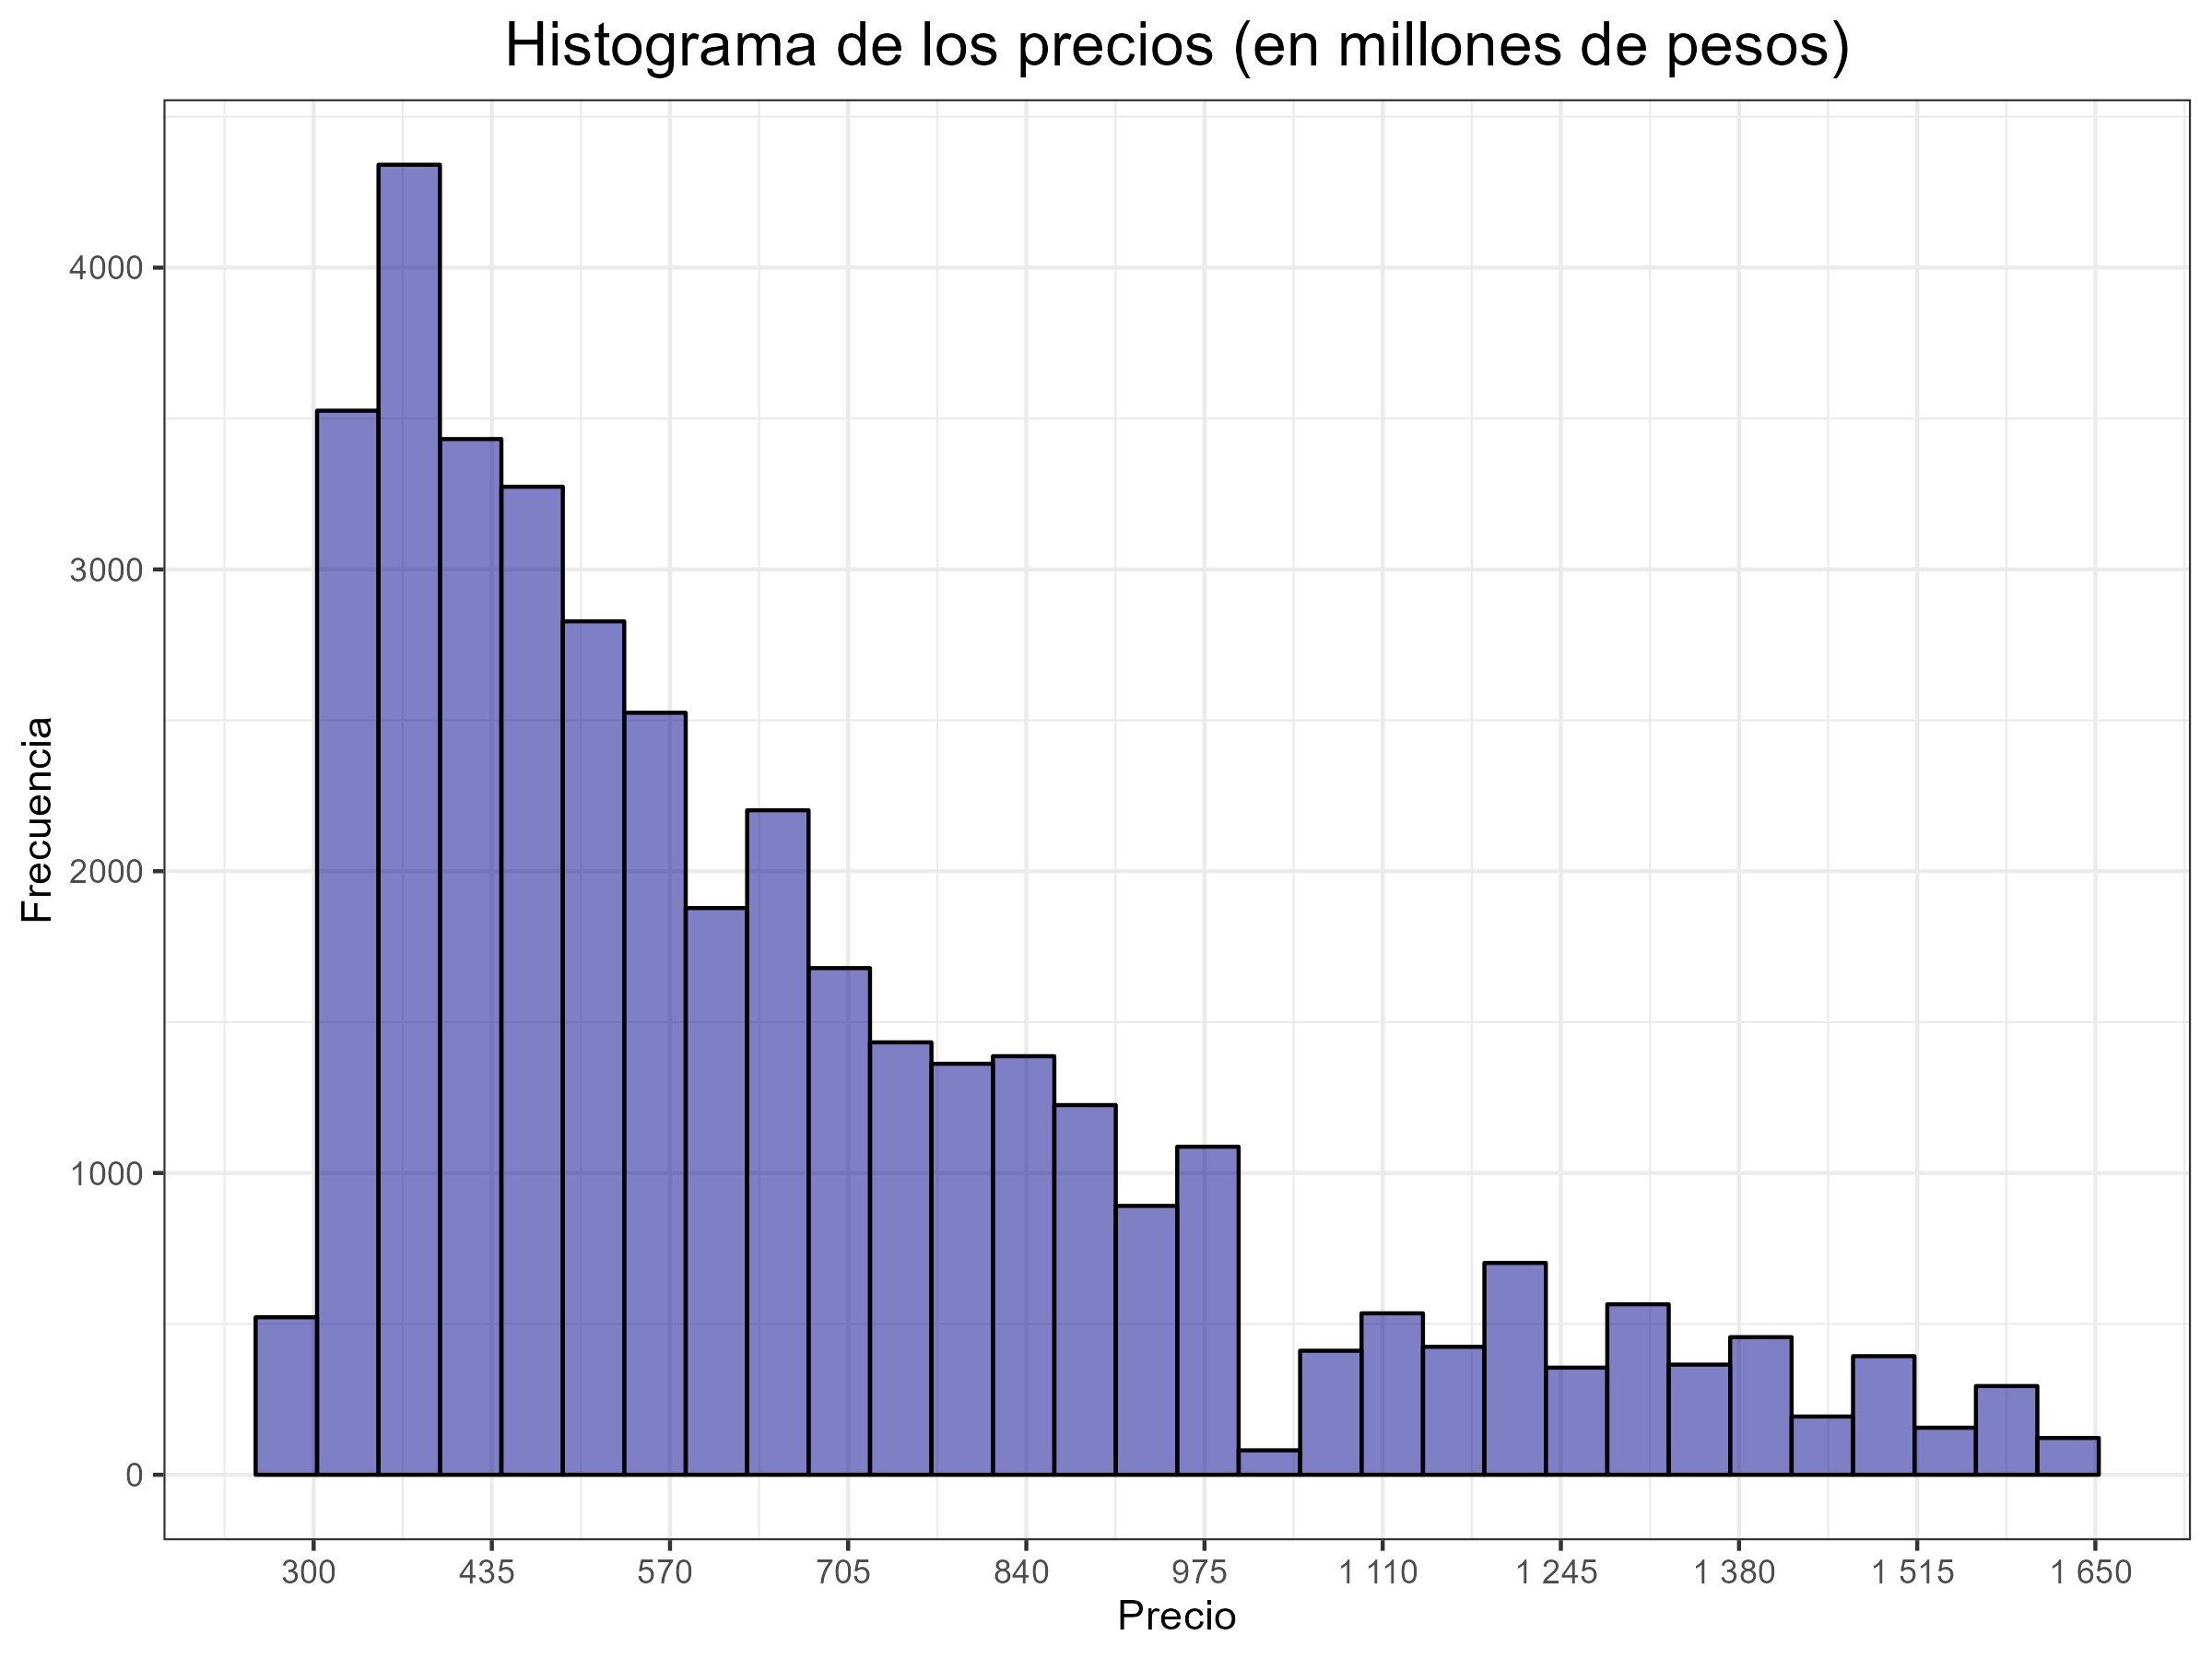
\includegraphics[scale=0.8]{../views/graficas_descriptivas/histograma_precio.png}
\centering
\caption{Distribución del precio de la vivienda en el grupo de datos de entrenamiento}
\label{fig:distribucion}
\end{figure}

El precio promedio de las viviendas en este conjunto es de aproximadamente 654.534.700, lo que da una idea del costo típico de una vivienda. Sin embargo, es esencial considerar la mediana, que se sitúa en 559.990.000, un valor ligeramente inferior al promedio. Esta diferencia entre la media y la mediana refleja el efecto de las viviendas de alto precio en la media, elevándola (ver anexo). \\

Otras variables importantes que nos gustaría revisar son las variables espaciales, para lo cual nos centraremos solamente en dos de ellas: la distancia mínima de cada observación a un parque, y la distancia mínima de cada observación a una estación de transmilenio. 

En la Gráfica \ref{fig:distribucion_tm} se puede observar un sesgo a la derecha, denotando que en el set de datos, la mayoría de propiedades se encuentran a una distancia de 2km (2000m) o menos de una estación de transmilenio. Este comportamiento concuerda con lo esperado, dado que la localidad de chapinero tiene una gran cantidad de puntos para transporte público, especificamente las estaciones de transmilenio ubicadas en la Avenida Caracas. Por lo que se supondría que hay una mayor cantidad de viviendas en un radio espacial de 2km de esta avenida, en comparación a propiedades de 2 a 4km de distancia de estas.\\


Continuando con el análisis, nos gustaría mostrar los mapas correspondientes a algunos de los predictores que se consideran de los más relevantes. Una de las características fundamentales para la determinación de los precios de las viviendas, como se mencionó anteriormente, es el acceso a medios de transporte. A continuación se muestran los mapas para las estaciones de transmilenio (Gráfico \ref{fig:mapatransmi}) e SITP (Gráfico \ref{fig:mapasitp}) , como se mencionó previamente, la Avenida Caracas parece ser punto determinante para el acceso a transporte de transmilenio y en donde se concentran la mayoría de propiedades. Por otra parte, analizando el mapa de estaciones de SITP puede encontrarse mayor variabilidad, dado que hay una mayor cantidad de estos puntos en la localidad, por lo que las distancias mínimas de los predios a ellas serán mucho menores en relación a las de transmilenio y pueden no ser tan signifcativas sen la predicción de los precios (dado que la mayoría de los precios tienen alguna estación cerca). \\

Para finalizar, es preciso observar el mapa de ubicaciones de parques (Gráfico \ref{fig:mapaparques}), este también puede denotar divergencias en los precios de las viviendas, dado que para muchos individuos es relevante la cercanía a estos puntos dado que tienen mascotas o niños, cuestión que puede añadir valor agregado a las propiedades.\\

\begin{figure}[H]
\centering
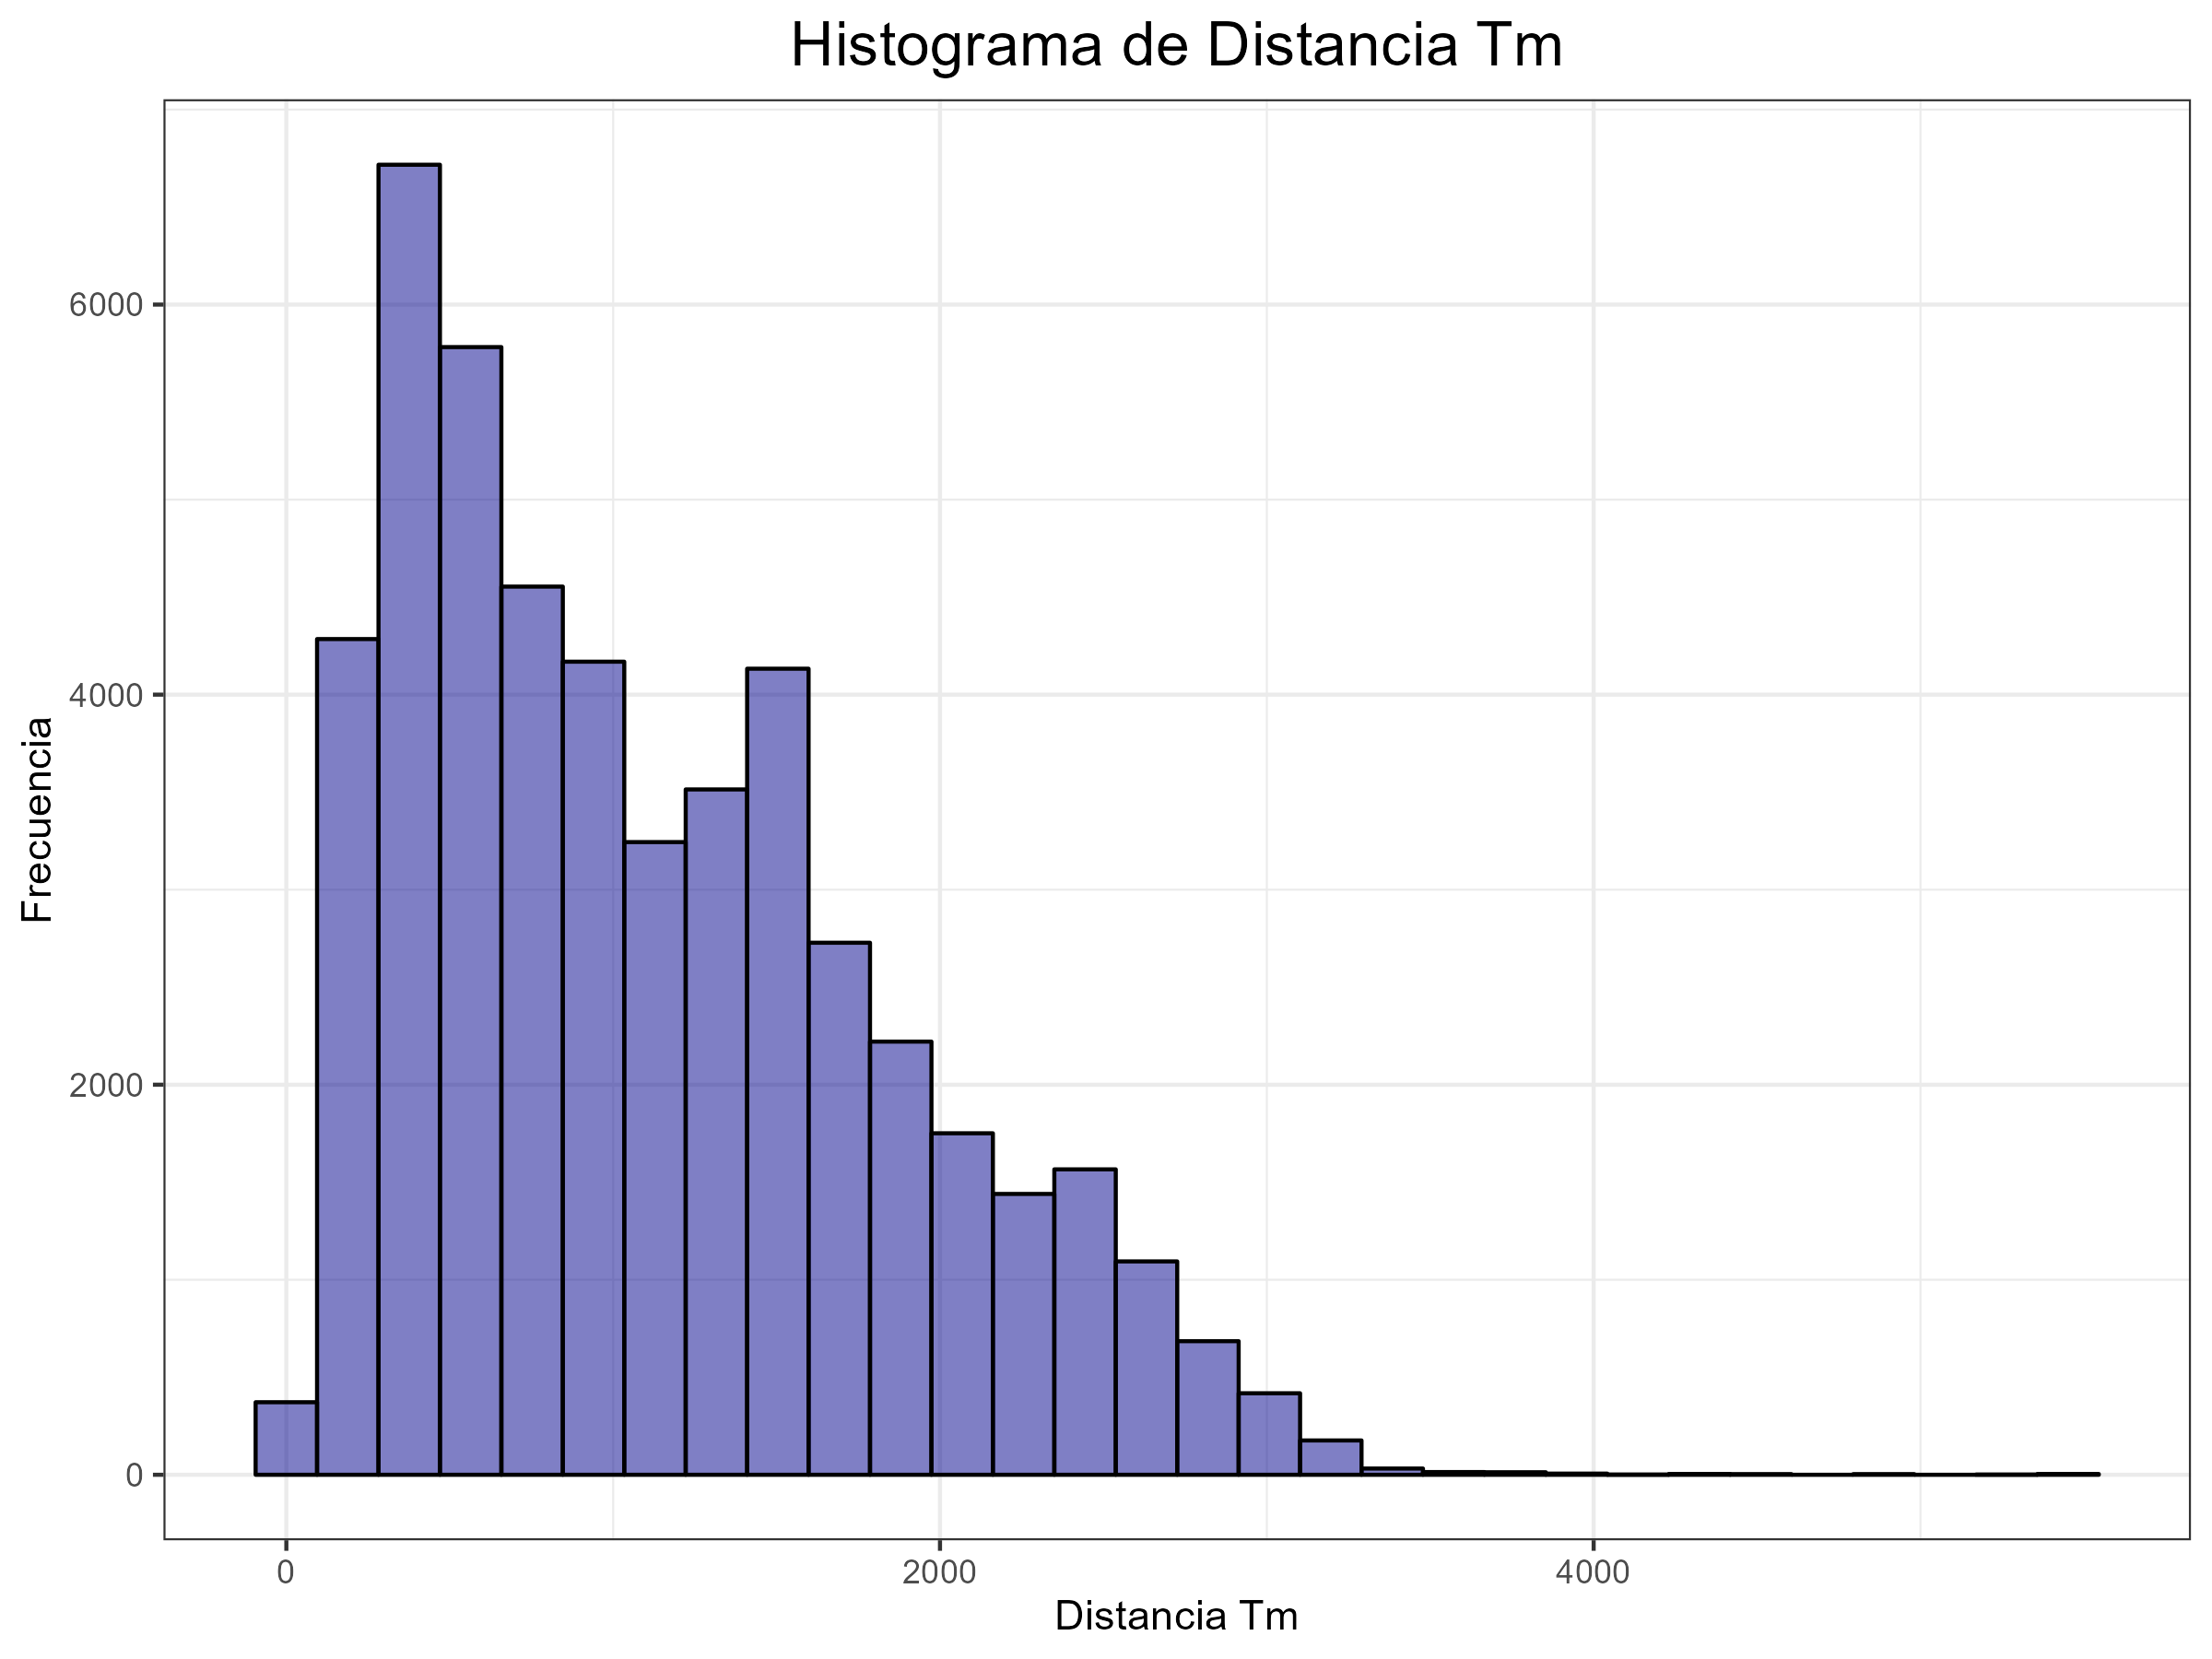
\includegraphics[scale=0.8]{../views/graficas_descriptivas/histograma_distancia_tm.png}
\centering
\caption{Distribución de la distancia minima a una estacion de transmilenio}
\label{fig:distribucion_tm}
\end{figure}

\begin{figure}[H]
    \centering
    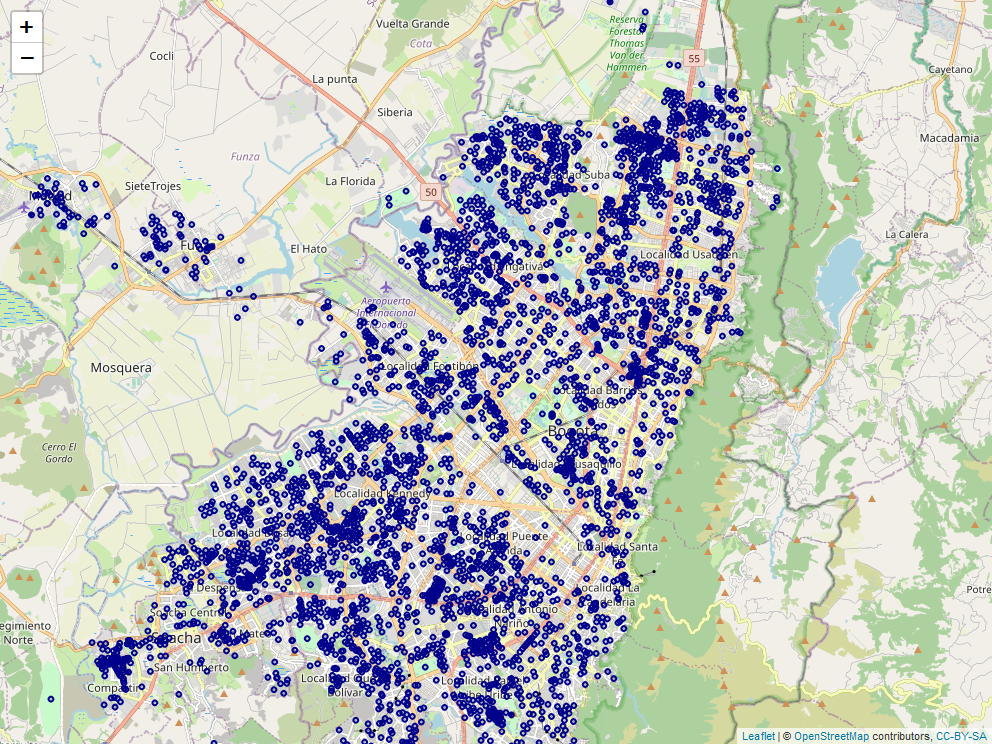
\includegraphics[scale=0.50]{../views/mapas/park.png}
    \caption{Mapa con parques siguiendo Open Street Maps}
    \label{fig:mapaparques}
\end{figure}
\begin{figure}[H]
    \centering
    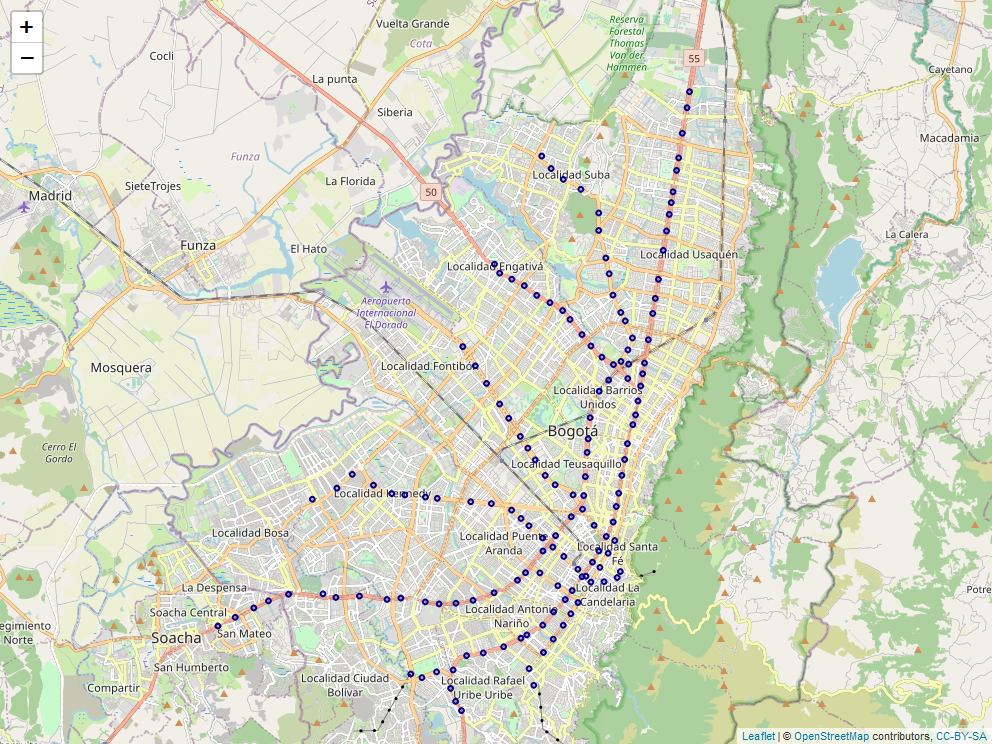
\includegraphics[scale=0.50]{../views/mapas/transmilenio.png}
    \caption{Mapa con estaciones de transmilenio.}
    \label{fig:mapatransmi}
\end{figure}

\section{Modelo y Resultados}
En esta sección presentamos el modelo que tuvo un mejor poder de predicción de los precios de las vivienda.

\subsection{Variables Utilizadas}
\begin{itemize}
    \item \textbf{Variables Numéricas (10)}: Rooms, Bathrooms, Piso\_numeric, Surface\_2, \\
    Area\_residencial\_manzana, valor\_catastral\_referencia\_2022,\\ numero\_predios\_manzana, nombre\_localidad, area\_construida\_residencial\_predio, valor\_catastral\_vivienda.
    \item \textbf{Variables Cualitativas (Factores/Dummy) (8)}: Utilizamos la variable de descripción para obtener, a través de procesamiento de lenguaje natural, variables que indiquen si una determinada vivienda cuenta con servicios importantes para predecir el precio, tales como: Parqueadero, Terraza, Ascensor, Vigilancia, Depósito, Cocina Integral y Piso Laminado. El tipo de propiedad se extrajo directamente de la base de datos.
    \item \textbf{Variables de Distancia}: En R utilizamos datos de Open Street Maps para obtener la ubicación de varios servicios y actividades de ocio, y calcular la distancia mínima a cada uno de estos servicios para cada observación. También incluimos datos de las estaciones de transmilenio y sitp de datos abiertos de Bogotá.

    Asimismo, se incluyeron polys de grado 3 para las variables de distanci en los algoritmos de boosting, lasso-boosting y regresión lineal. Estos 3 siendo los de mejor rendimiento entre todos los intentos subidos a kaggle.
\end{itemize}
    
\subsection{Modelo de predicción}

Utilizar la metodología de Boosting generó la mejor propuesta del presente estudio con una puntuación de 210'699.544 (Naus, 2023). Es decir, el modelo predice los precios para viviendas en Chapinero con un error de \$210’699.554 COP. Las variables numéricas y cualitativas mencionadas previamente plantean un enfoque hedónico el cual nos permite capturar el valor monetario de las características individuales de los inmuebles. Paralelamente, dicho enfoque es complementado haciendo uso de las variables de distancia. Estas permiten incorporar diferentes interacciones entre el precio de un inmueble y su cercanía con diferentes amenities en la ciudad.\\

Es importante destacar que, para todos los modelos, implementamos validación cruzada mediante pliegues (k-folds), estableciendo en la mayoría de los casos un total de 10 pliegues ($k=10$). Sin embargo, dada la naturaleza de los datos y la potencial autocorrelación espacial entre las observaciones, recurrimos a la Validación Cruzada Espacial con el objetivo de optimizar las predicciones de los modelos.

La selección del modelo tuvo un componente teórico importante. Para comenzar, el boosting construye un modelo de predicción robusto a partir de un conjunto de árboles de decisión débiles. Cada árbol es entrenado iterativamente teniendo en cuenta sus predecesores con el objetivo de aprender y corregir errores previos dando mayor relevancia a instancias mal clasificadas. Como resultado de esto, en segundo lugar, este modelo tiene la capacidad de reducir la varianza y mejorar la consistencia del modelo. Por si fuera poco, el boosting puede controlar el problema de sobreajuste típico de los árboles de decisión ya que limita la profundidad de estos.\\

 Los precios de las viviendas suelen estar influenciados por una variedad de factores, algunos de los cuales pueden tener relaciones no lineales o interacciones complejas. El modelo de boosting puede capturar estas relaciones de manera efectiva al combinar múltiples modelos débiles en uno fuerte, lo que le permite modelar de manera más precisa las relaciones entre las características de las viviendas y sus precios. \\ 
 
En nuestro caso particular, los hiperparametros del modelo fueron optimizados planteando una grilla (ver Table 3), estos rangos de valores fueron escogidos después de hacer diversas pruebas y encontrar que en repetidas ocasiones los valores eran cercanos a los denotados en esta tabla. Por ejemplo, dos boosting previos con peor rendimiento, habían mejorado la puntuación de kaggle con profundidades de árbol de 1 para ambos, con 120-122 árboles y tasas de aprendizaje en rangos cercanos a 1. Lo que hicimos fue acotar la grilla a estos valores para poder acercarse más a aquellos hiperparámetros que fueran más adecuados para la predicción 

Por lo anterior, se propone un rango de número de árboles que inicia en 100 y finaliza en 130. El mejor modelo se encuentra con 114 árboles, cada uno con una profundidad de 1. En otras palabras, esta elección se traduce en un modelo final compuesto por una ponderación de árboles simples y poco profundos. Finalmente, la elección de la tasa de aprendizaje del modelo se derivó de una grilla propuesta que tenía un rango desde 0.001 a 0.005. Sin embargo, los resultados sugieren que la mejor tasa de aprendizaje encontrada fue de 1.008 y 20 niveles. De esta manera, si bien el modelo de boosting propone un equilibrio entre la robustez y la interpretabilidad del modelo para la predicción de precios de los inmuebles, futuros estudios pueden enfocarse en encontrar una tasa de aprendizaje más lenta que el modelo propuesto en este estudio.\\

    \begin{table}[ht]
    \centering
    \begin{tabular}{lccc}
    \hline
    Hiperparámetro & Límite inferior & Límite superior & Parámetro elegido \\
    \hline
    Árboles (tree) & 100 & 130 & 114 \\
    Profundidad de árbol (tree\_depth) & 1 & 1 & 1  \\
    Tasa de aprendizaje (learn\_rate) & 0.001 & 0.005 & 1.008153  \\
    Niveles(levels) &  &  & 20  \\
    \hline
    \end{tabular}
    \caption{Elección de hiperparámetros}
    \end{table}


\subsection{Evaluación del modelo de predicción}

A manera comparativa, la Tabla 4 resume las mejores predicciones de cada uno de los modelos propuestos en el presente estudio. Para comenzar, el segundo mejor modelo se obtuvo de estimar los precios de las viviendas combinando los modelos de Boosting y Lasso.  El primero de ellos, permite mejorar la precisión del modelo combinando diferentes modelos débiles que aprenden de manera iterativa. En paralelo, esto se compensa con la técnica de regularización L1 de Lasso que permite reducir la complejidad del modelo y, así, evitar el sobreajuste (eliminar predictores no necesarios). Esta combinación de características pudo ser la clave para que este modelo quedará en segundo lugar. \\

Sin embargo, por si solos estos modelos quedan en peores posiciones. Por su parte, Lasso pierde la capacidad de autoaprendizaje de Boosting y queda en el quinto puesto. Similarmente, Boosting queda en el noveno puesto posiblemente debido a que cae en el sobreajuste de la muestra y, por tanto, pierde capacidad predictiva fuera de ella debido a la ausencia de Lasso. \\

De manera similar, el modelo Ridge que utiliza el método de regularización L2 para reducir la complejidad de los modelos reduciendo el riesgo de sobreajuste queda en el cuarto puesto. Esto sugiere que Lasso es más efectivo reduciendo el modelo estimado, para el caso particular de nuestros datos, lo cual tiene beneficios en términos de predicción fuera de muestra. Ahora bien, llama la atención que el modelo estimado mediante Eslastic Net quedara en la sexta posición. Si bien este utiliza tanto las técnicas de regularización L1 y L2 para reducir los modelos y evitar su sobreajuste, la característica de aprendizaje del modelo de Boosting puede ser el detonante del mal desempeño comparado de Elstic Net respecto a otros modelos. \\

Por otro lado, Random forest y Árboles de decisión se encuentran en las posiciones sexta y séptima, respectivamente. Ambos modelos son entrenados en subconjuntos aleatorios de prueba de las características de los inmuebles. La razón por la cual ambos modelos quedaron en posiciones tan bajas de nuestra comparación es el sobreajuste al que tienden este tipo de modelos. Así, aunque tengan buenas predicciones en los subconjuntos de entrenamiento, fuera de muestra, los modelos pierden capacidad predictiva. Asimismo, cabe aclarar que estos intentos no incluían la misma cantidad de variables que tuvo el Boosting con mejor score, razón por la cual pudieron tener este rendimiento tan bajo.\\

Finalmente, en segundo lugar se posiciona el modelo de regresión lineal. Llama la atención su capacidad de predicción teniendo en cuenta que es uno de los modelos más sencillos utilizados en machine learning. En este caso particular, la forma funcional propuesta se ajusta de manera adecuada a los datos y, al tiempo, plantea predicciones valiosas para el presente estudio, a este modelo se le incluyeron las mismas variables que el boosting con mejor score, es decir, variables cualitativas, cuantitativas, de distancia, interacción y polys de grado 3 para las variables distancia . Adicionalmente, una ventaja comparativa del modelo de regresión líneal es su interpretabilidad, sin embargo, no se realizará esta interpretación, dado que hay más de 200 estimadores.\\

    \begin{table}[ht]
    \centering
        \begin{tabular}{lcccccc}
        \hline
        & \multicolumn{5}{c}{Hiperparámetros} &\\
        \cline{2-6}
        Modelo & Penalty & Mixture & Trees & Tree Depth & Learn Rate & Score \\
        \hline
        Boosting & & &114 & 1& 1.0082 & \$210.699.554,89 \\        
        Lasso boosting & 0.001 & & 140 & 1 & 0,8723 & \$214.741.670,84\\
        Linear regression & & & & & & \$232.644.942,35 \\
        Ridge & 0.0723 & & & & &\$241.605.005,24 \\
        Lasso & 0.001 & & & & & \$254.010.725,29 \\
        Elastic net & 0.0062 &0.596& & & & \$256.385.454,00 \\
        Decision tree &  & & & 8 & & \$291.599.337,79 \\
        \hline
        & \multicolumn{5}{c}{Hiperparámetros} &\\
        \cline{2-6}
        & \multicolumn{2}{c}{mtry} & Trees & \multicolumn{2}{c}{No. min observaciones} & Score \\
        Random Forest & \multicolumn{2}{c}{4} & 110 & \multicolumn{2}{c}{10} & \$282.603.449,10 \\
        \hline
        \end{tabular}
        \caption{Mejores resultados de predicción por tipo de modelo}
    \end{table}


\section{Conclusiones y recomendaciones}

El modelo  boosting es una opción poderosa y versátil para predecir precios de vivienda debido a su capacidad para capturar relaciones complejas en los datos; su resistencia a datos faltantes y valores atípicos; y su rendimiento generalmente sólido en una variedad de escenarios. Sin embargo, es importante destacar que el éxito del modelo depende de la calidad de los datos y la correcta selección de hiperparametros. \\

En el presente trabajo se utilizaron cerca de 148 predictores, esta situación puede considerarse problemática, sin embargo, al realizar un depuración de las variables con lasso y después correr un boosting, se encontró que la predicción del modelo empeoraba, por lo que se considero relevante mantener esta cantidad de predictores y poder capturar la mayor cantidad de información disponible.\\

Por otro lado, la empresa debe hacer una inversión inicial en recolectar datos que permitan construir predictores sobre las valoraciones de localización, proximidad , calidad urbana y condiciones financieras de la vivienda que hacen que los propietarios asignen mayores precios a la vivienda. La disponibilidad de este tipo de datos garantiza mejorar la capacidad de predicción especialmente en un mercado tan sensible a las fluctuaciones de los ingresos de los hogares. \\

En ese sentido, es recomendable que la organización pueda implementar modelos de predicción dirigidos a: (a) reducir la complejidad dado la cantidad de características que determinan el precio de la vivienda, (b) el tratamiento de los datos atípicos e irregulares que son propios del mercado de la vivienda y (c) tener una sistematización  sobre el aprendizaje de la selección de hiperparametros.\\


\section{Referencias}
Cabrera-Rodríguez, W., Mariño-Montaña, J. y Quicazán-Moreno, C. (2019). Modelos Hedónicos con Efectos Espaciales: Una Aproximación al Cálculo de Índices de Precios de Vivienda para Bogotá. Borradores de Economía.\\

James, G.,Witten, D.,Hastie, T., y Tibshirani, R. (2021). Tree-Based Methods en James, G.,Witten, D.,Hastie, T., y Tibshirani, R. (2021).  An Introduction to Statistics with Applications in R (pp. 327 – 361). Springer.\\

Naus. (2023). Uniandes BDML 2023\_20 PS2. Kaggle. Recuperado de \url{https://kaggle.com/competitions/uniandes-bdml-202320-ps2}

\section{Anexo: Gráficas Descriptivas}

\begin{figure}[ht]
    \centering
    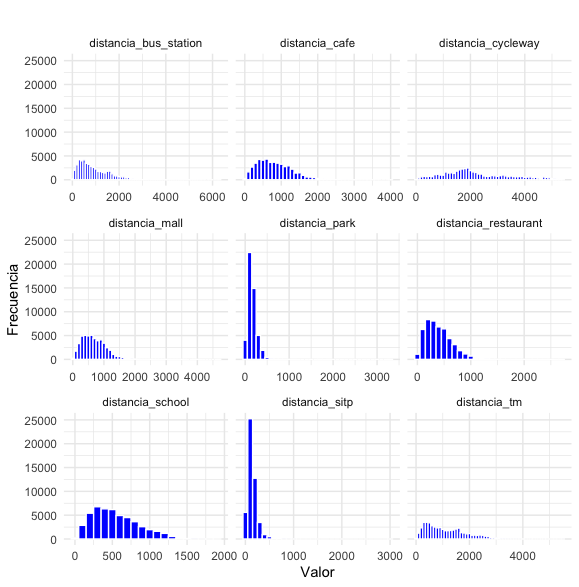
\includegraphics[scale=0.6]{../views/graficas_descriptivas/Histograma_distancias.png}
    \caption{Distancia promedio a servicios y equipamientos}
\end{figure}

\begin{figure}[ht]
    \centering
    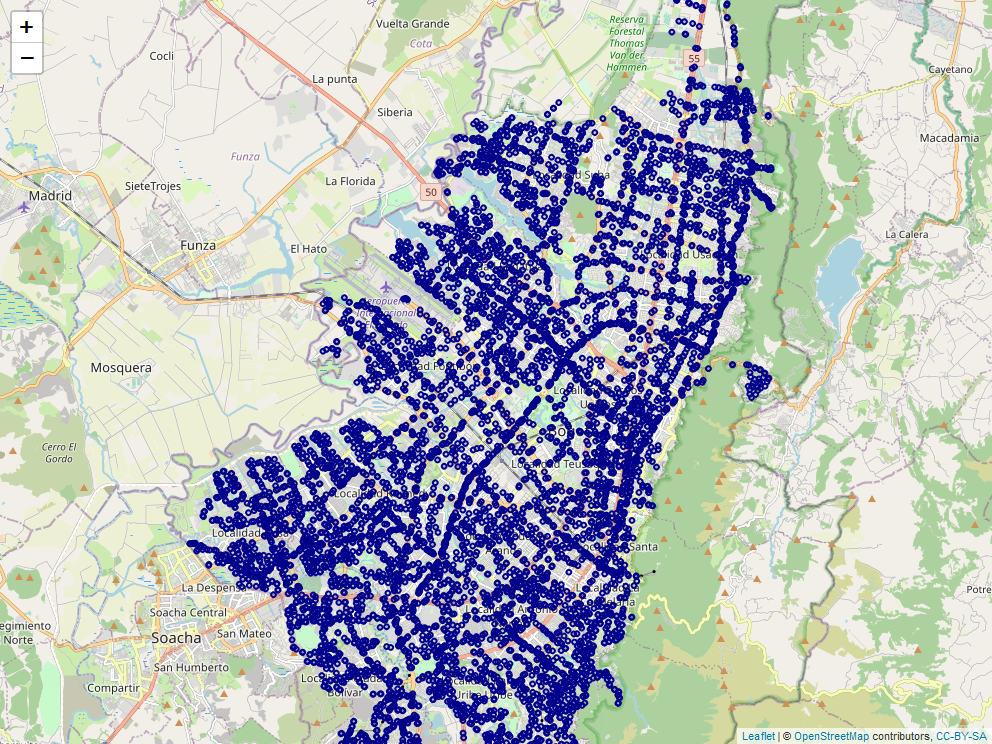
\includegraphics[scale=0.50]{../views/mapas/sitp.png}
    \caption{Estaciones de SITP}
    \label{fig:mapasitp}
\end{figure}

\end{document}
